%!TEX program = xelatex

\documentclass[12pt]{ctexbeamer}

%草本
	%draft;不含背景等,加快编译速度
%挑选一些frame编译
	%\includeonlyframes{example1}
	%\frame[label=example1] {This frame will be included. }
%缩印本
	%\usepackage{pgfpages}
	%\pgfpagesuselayout{4 on 1}[a4paper,border shrink=5mm,landscape]%resize to; 2 on 1; 4 on 1
\usepackage[ustcblue]{ustcbeamer}%可通过更改选项来更改主题颜色

%%%模板说明%%%%
%模板ustc_beamer中定义了五个选项供选择:ustcblue,ustcred,black,violet,blue;分别对应了五种主题颜色。
%建议使用ustcblue和ustcred,两者均为科大党委宣传部规定的校徽标准配色,参考http://lswhw.ustc.edu.cn/index.php/index/info/3370 。两个标准配色分别为:蓝cmyk(100,80,0,0)、红cmyk(0,100,100,0),在LaTex中使用需要除以100。
%本模板参考了https://github.com/thomasWeise/ustcSlides 的Slides,故而保留了Thomas Weise先生的原始配色(blue)。
%不怎么建议使用黑色(black),看上去像讣告。
%有其他的配色需求可在github上反馈。
%%%%%%%%%%%%%%%%%%%%%%%%%%%%%%%%%%%%%%%%%%%%%%%%%%%%%%%%%%%%%%%%%%%%%%


\title[底部简明标题]{
    关于基于网络的入侵检测系统的调查
}
\author[底部演讲者]{林静雯、胡冬寅、李锭轩}
\institute[USTC]{
中国科学技术大学,信息安全系
}
\date{2019年6月6号}
\begin{document}
%\section<⟨mode specification⟩>[⟨short section name⟩]{⟨section name⟩}
%小于等于六个标题为恰当的标题

%--------------------
%标题页
%--------------------
\maketitleframe
%--------------------
%目录页
%--------------------
%beamer 101
\begin{frame}%
	\frametitle{大纲}%
	\tableofcontents[hideallsubsections]%仅显示节
	%\tableofcontents%显示所节和子节
\end{frame}%
%--------------------
%节目录页
%--------------------
\AtBeginSection[]{
\setbeamertemplate{footline}[footlineoff]%取消页脚
  \begin{frame}%
    \frametitle{大纲}
	%\tableofcontents[currentsection,subsectionstyle=show/hide/hide]%高亮当前节,不显示子节
    \tableofcontents[currentsection,subsectionstyle=show/show/hide]%show,shaded,hide
  \end{frame}
%\setbeamertemplate{footline}[footlineon]%添加页脚
}
%--------------------
%子节目录页
%--------------------
\AtBeginSubsection[]{
\setbeamertemplate{footline}[footlineoff]%取消页脚
  \begin{frame}%
    \frametitle{大纲}
	%\tableofcontents[currentsection,subsectionstyle=show/hide/hide]%高亮当前节,不显示子节
    \tableofcontents[currentsection,subsectionstyle=show/shaded/hide]%show,shaded,hide
  \end{frame}
%\setbeamertemplate{footline}[footlineon]%添加页脚
}

\section{导言}
\begin{frame}
  \frametitle{导言}
      \begin{figure}
        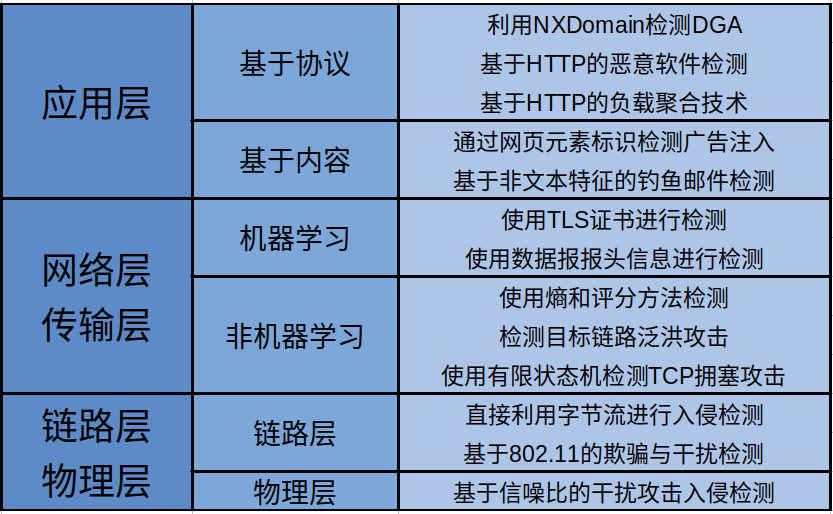
\includegraphics[width=0.8\textwidth]{figures/list_all.png}
 %       \caption{}
      \end{figure}
\end{frame}


\section{NIDS技术}
\subsection{应用层}
\begin{frame}
  \frametitle{鱼叉式钓鱼邮件检测}
  	\begin{figure}
    	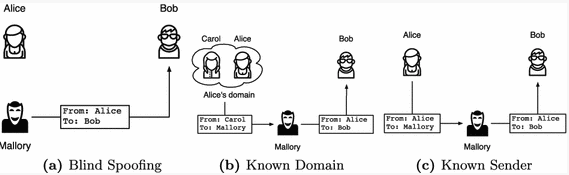
\includegraphics[width=1.0\textwidth]{figures/email_attack.png}
 %       \caption{鱼叉式钓鱼邮件攻击}
  	\end{figure}
%  \pause


\end{frame}



\begin{frame}
  \frametitle{鱼叉式钓鱼邮件检测}
  	\begin{figure}
    	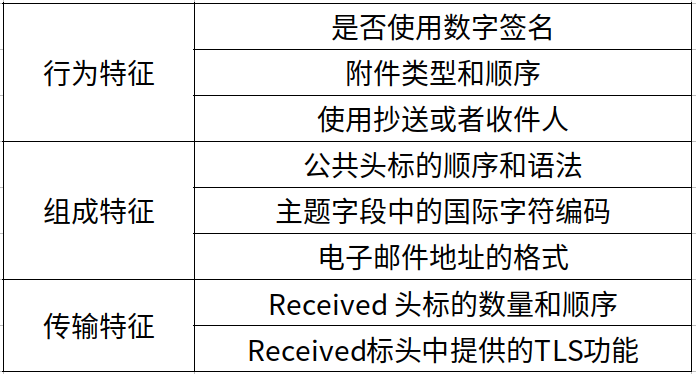
\includegraphics[width=0.8\textwidth]{figures/email2.png}
 %       \caption{基于非文本特征检测}
  	\end{figure}
%  \pause


\end{frame}





\subsection{网络层、传输层}
\begin{frame}
  \frametitle{机器学习方法}
  \begin{figure}
    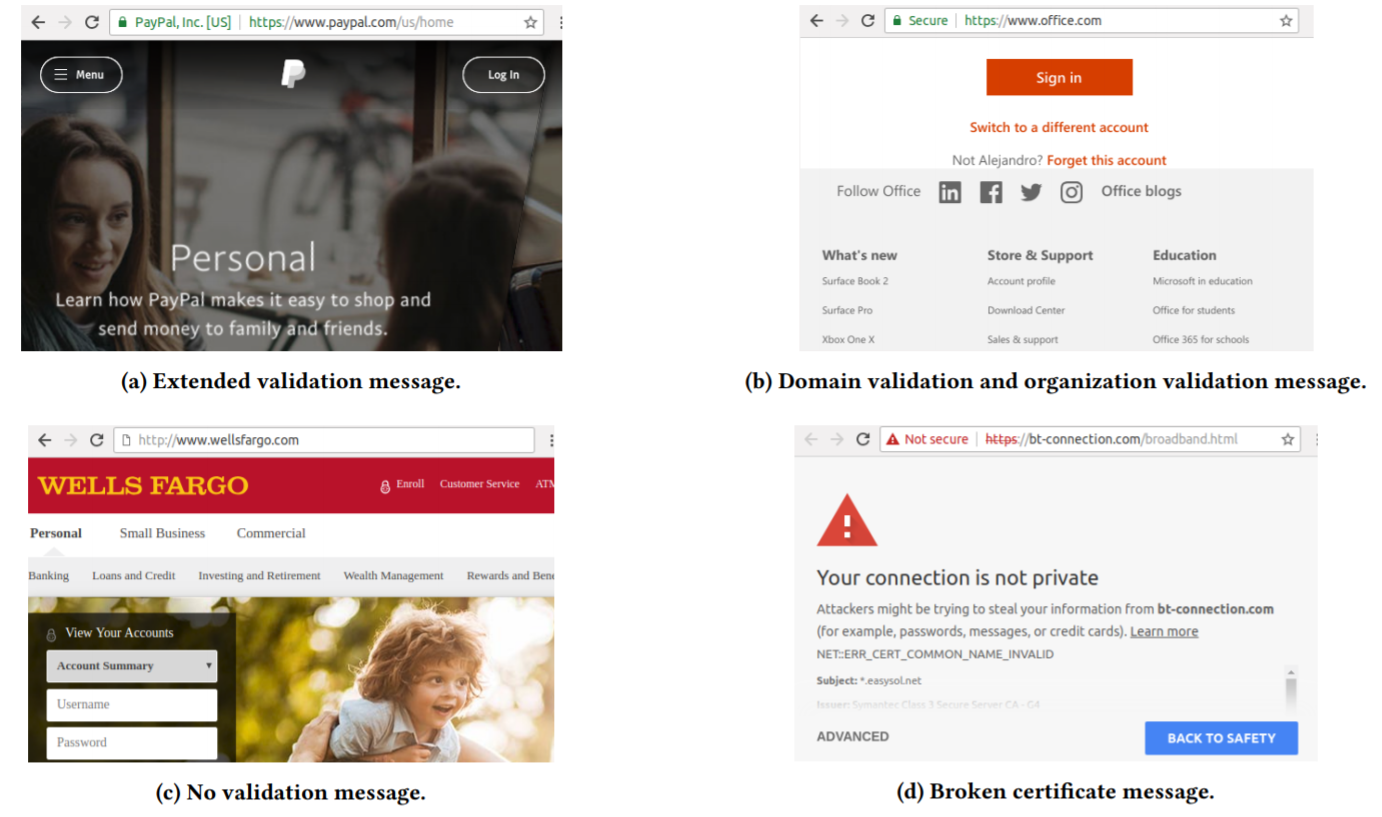
\includegraphics[width=10cm, height = 7.2cm]{figures/tls_cert.PNG}
%        \caption{使用KNN和SVM进行分类检测}
  	\end{figure}
%  \pause


\end{frame}

\begin{frame}
  \frametitle{机器学习方法}
  \begin{figure}
    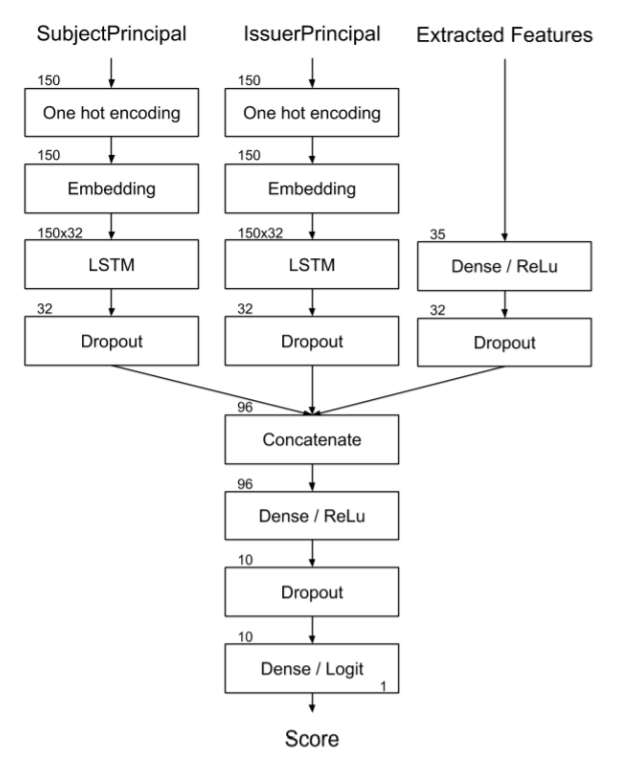
\includegraphics[width=7.3cm,height = 7.3cm]{figures/tls_block.PNG}
 %       \caption{使用KNN和SVM进行分类检测}
  	\end{figure}
%  \pause
 

\end{frame}

\begin{frame}
  \frametitle{非机器学习方法}
  \begin{figure}
    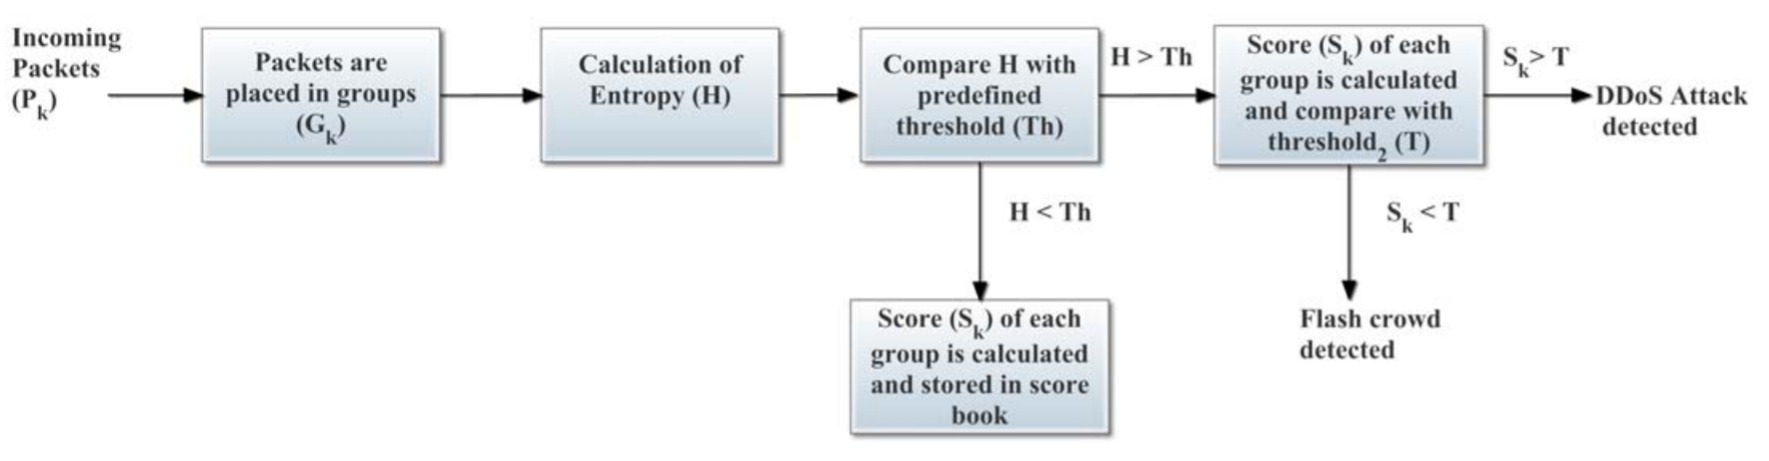
\includegraphics[width=1.1\textwidth]{figures/entropy.PNG}
%        \caption{使用KNN和SVM进行分类检测}
  	\end{figure}
%  \pause


\end{frame}

\subsection{链路层、物理层}
\begin{frame}
  \frametitle{利用字节流的入侵检测}
  \begin{figure}
    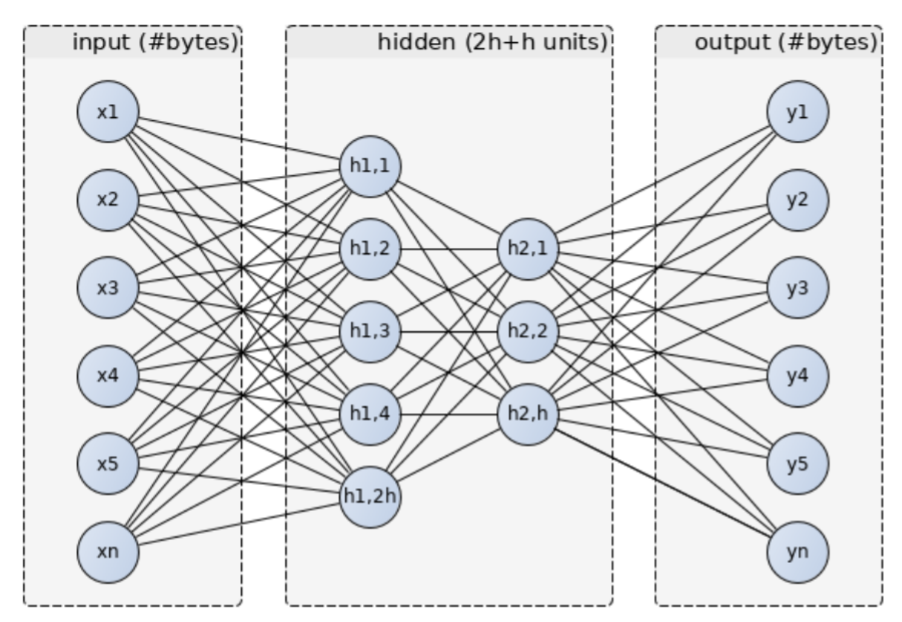
\includegraphics[width=0.85\textwidth]{figures/autoencoder.PNG}
%       \caption{使用KNN和SVM进行分类检测}
  	\end{figure}

\end{frame}



\section{未来方向}

\begin{frame}
  \frametitle{未来方向}
    \begin{itemize}
      \item 数据来源
      \item 面向连接型网络
      \item 协议栈各层
      \item NIDS检测的攻击类型
      \item 使用非统计方法
    \end{itemize}
\end{frame}

\begin{frame}
  \frametitle{数据来源}
  \begin{figure}
    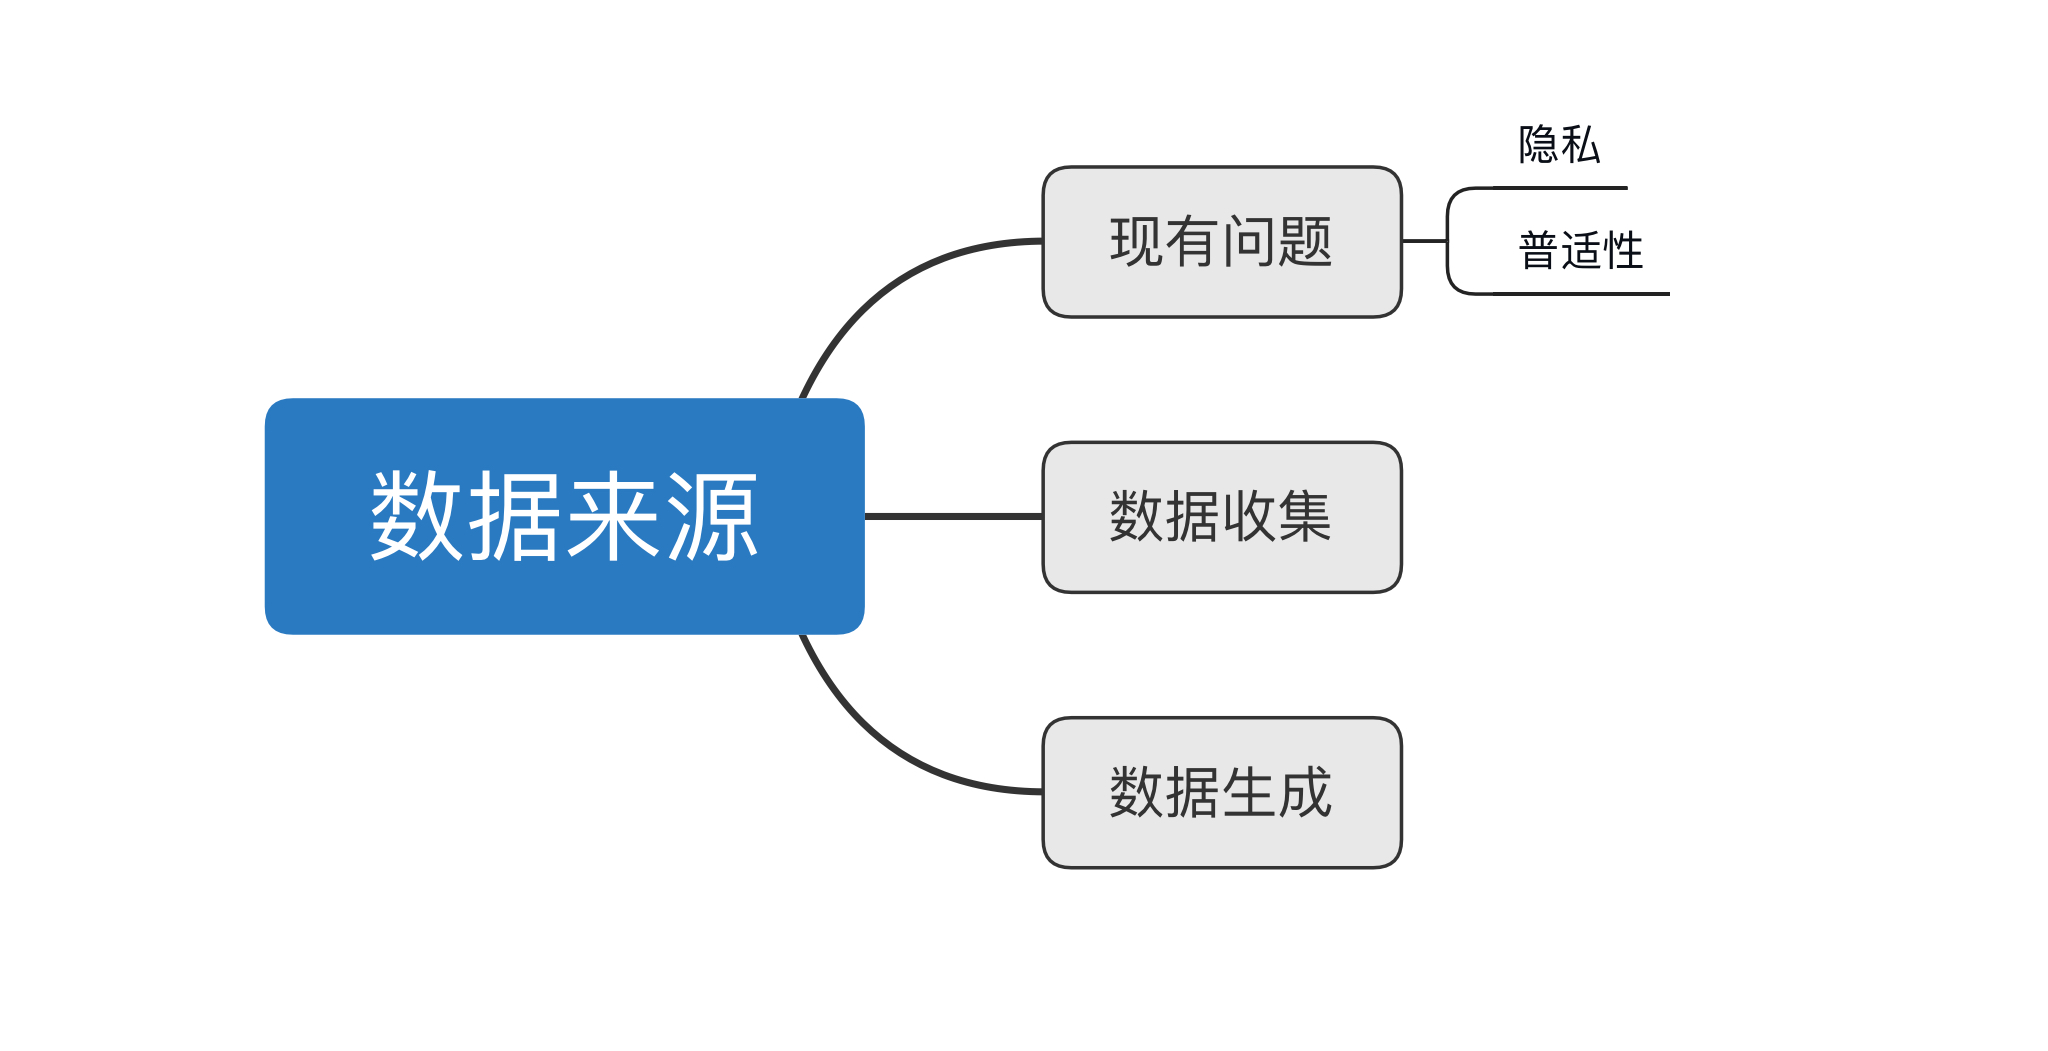
\includegraphics[width=1.0\textwidth]{figures/数据来源.jpg}
%        \caption{使用KNN和SVM进行分类检测}
  	\end{figure}

\end{frame}


\begin{frame}
  \frametitle{攻击类型}
  \begin{figure}
    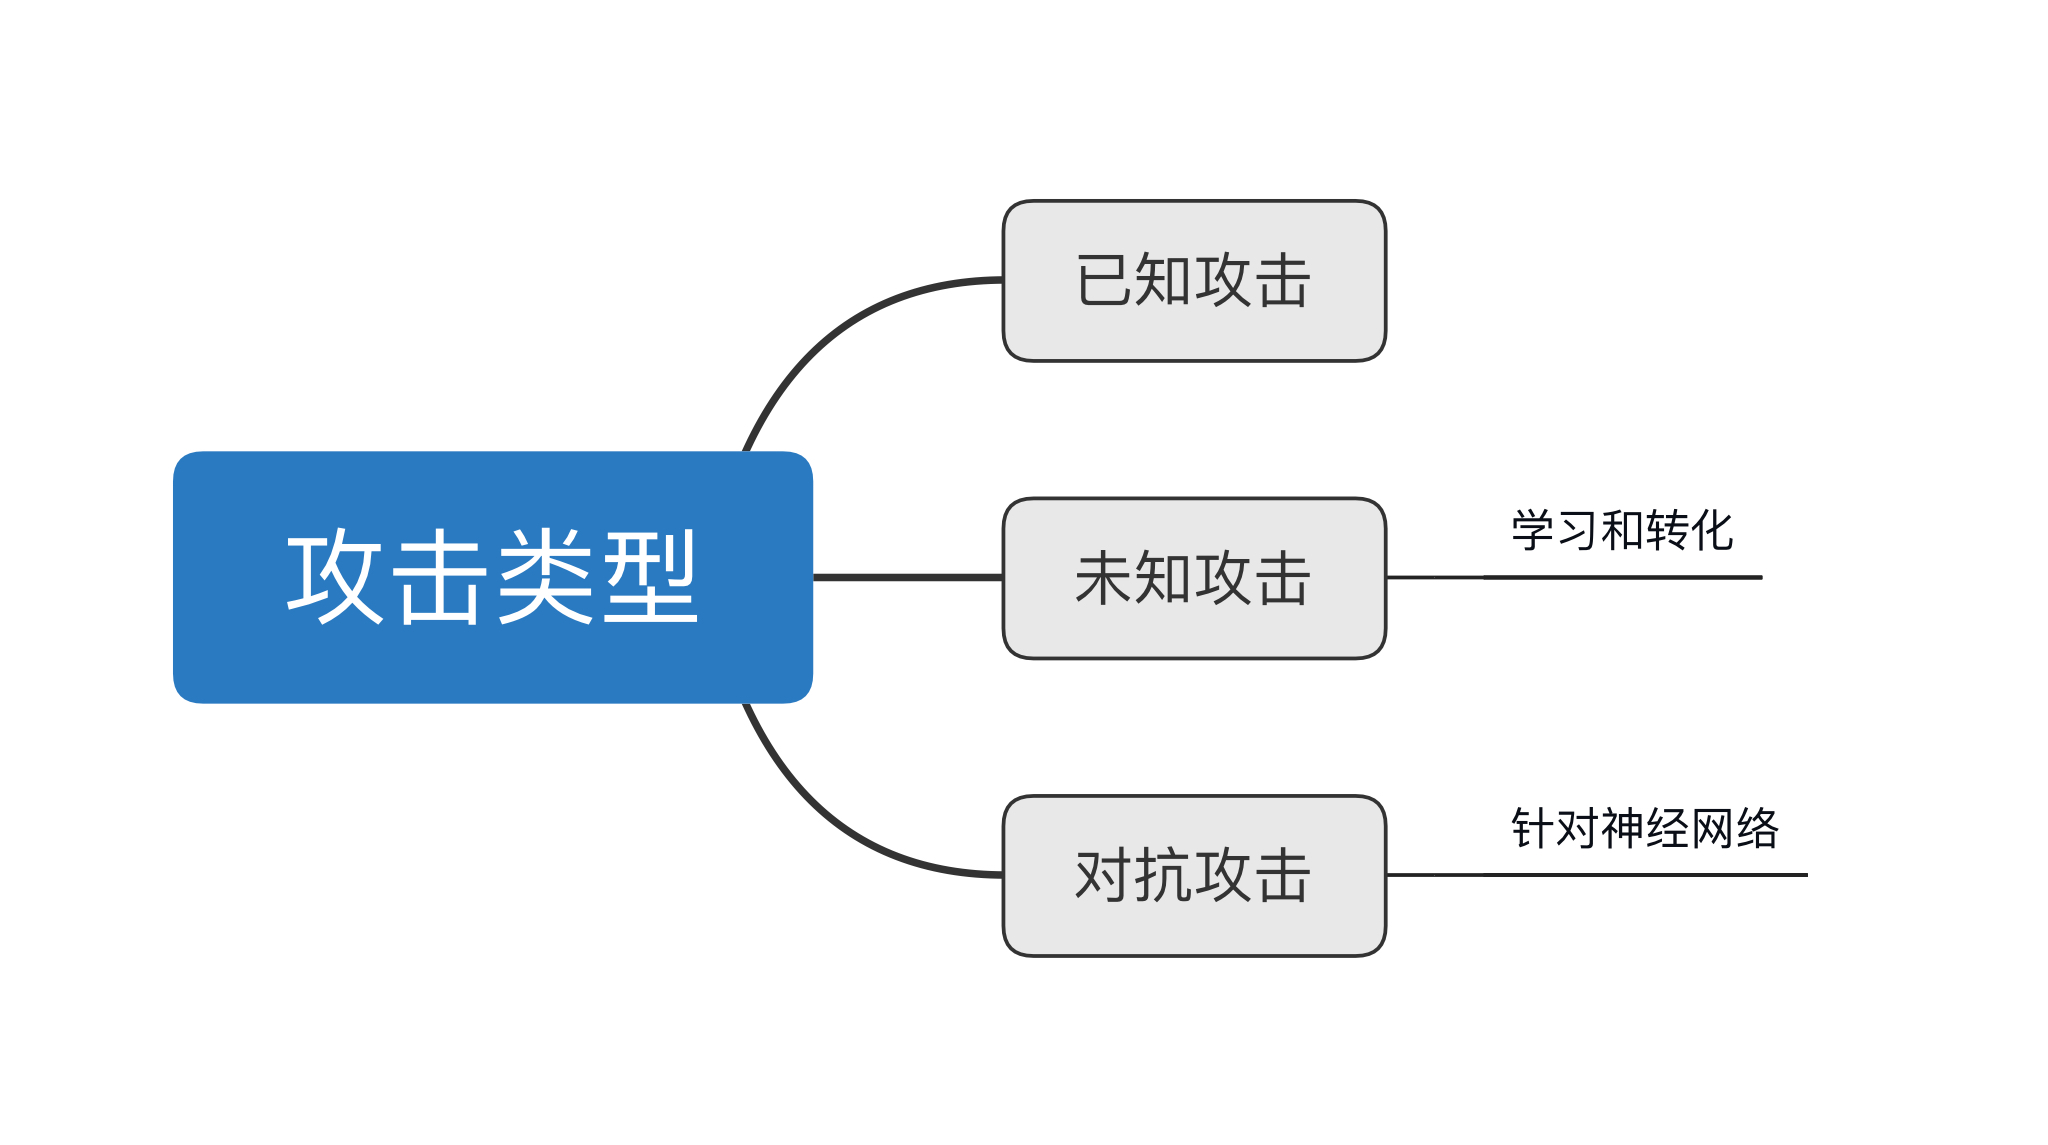
\includegraphics[width=1.0\textwidth]{figures/攻击类型.jpg}
%        \caption{使用KNN和SVM进行分类检测}
  	\end{figure}

\end{frame}


\begin{frame}
  \frametitle{非统计方法}
  \begin{figure}
    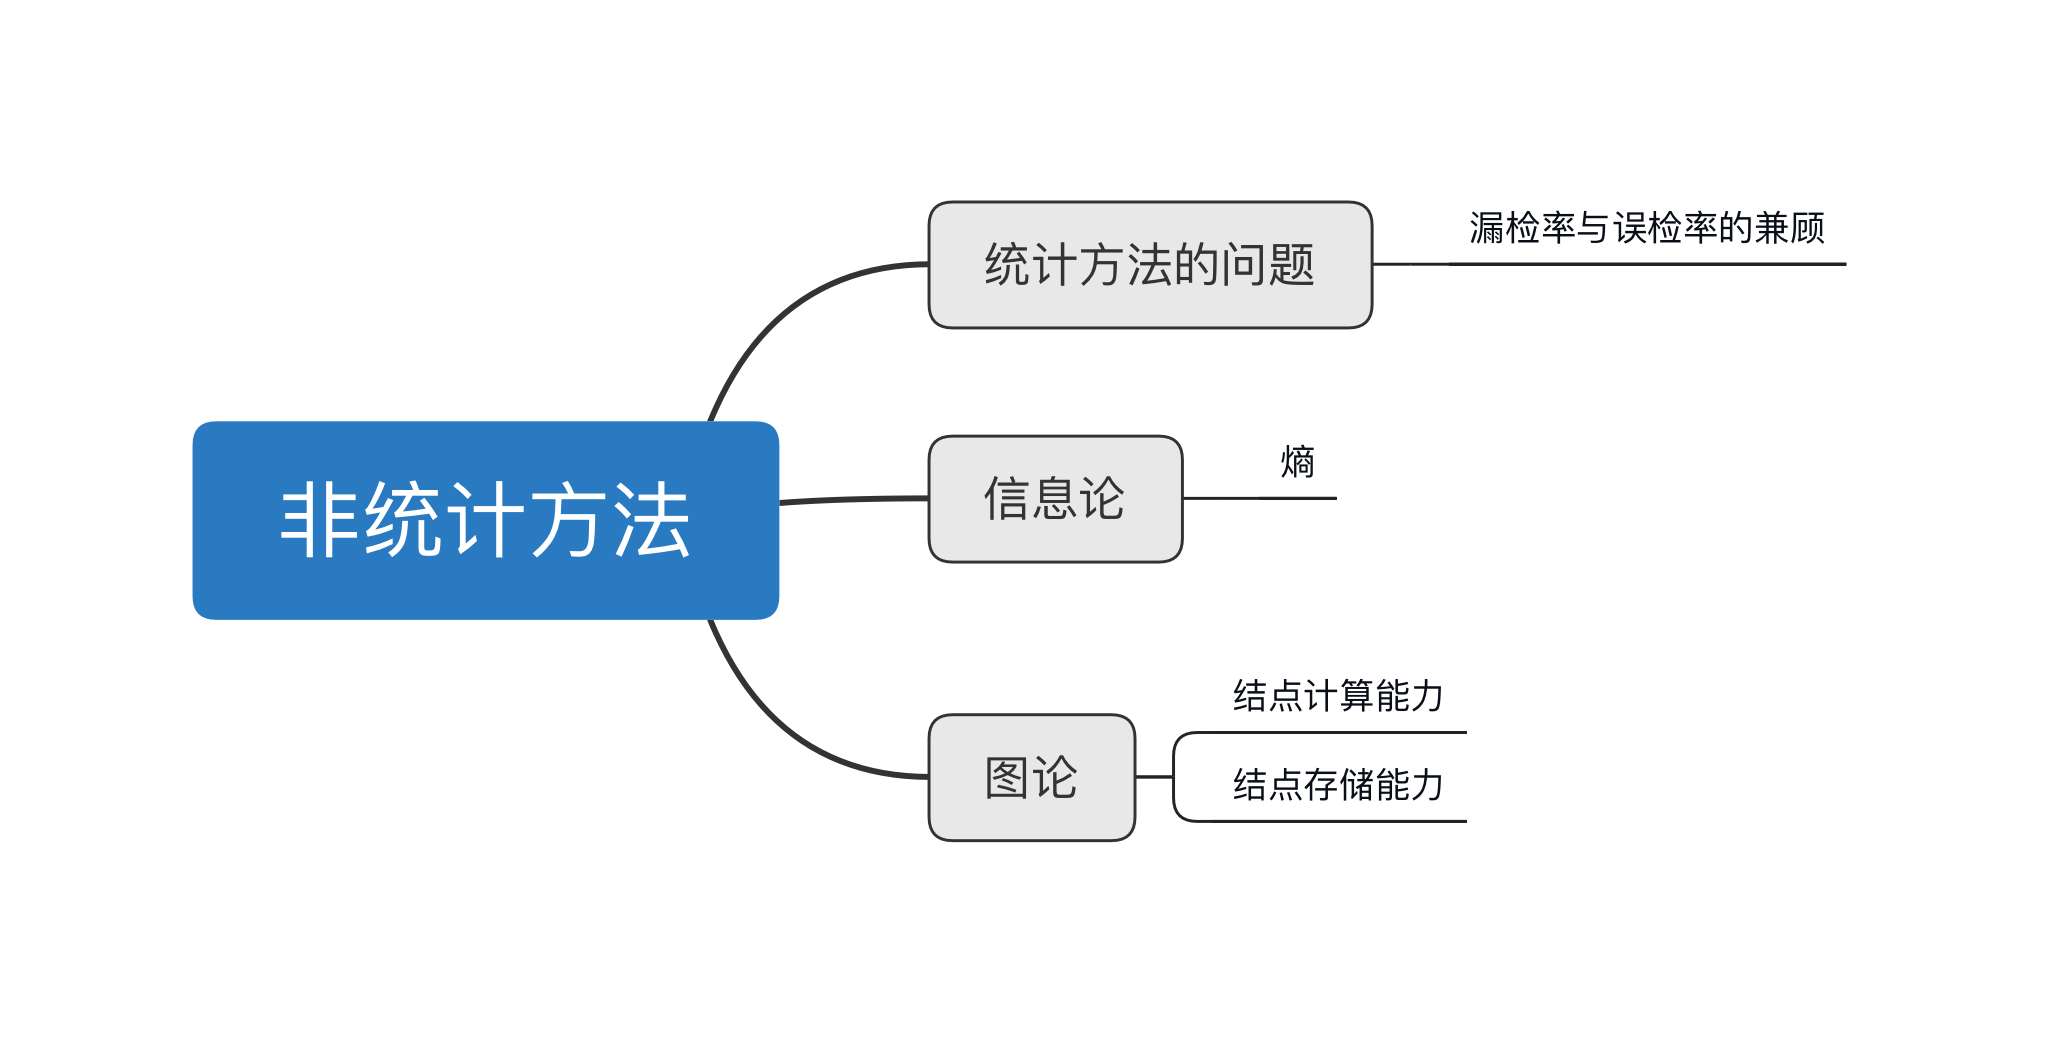
\includegraphics[width=1.0\textwidth]{figures/非统计方法.jpg}
%        \caption{使用KNN和SVM进行分类检测}
  	\end{figure}

\end{frame}

\begin{frame}
  \centerline{\Large 谢谢!}
\end{frame}

%
%\section{总结展望}
%
%\begin{frame}
%  \frametitle{总结展望}
%  \begin{columns}
%    \begin{column}{0.50\textwidth}
%      \begin{figure}
%        
\includegraphics[width=0.8\textwidth]{figures/ustc_logo.pdf}
%        \caption{标题}
%      \end{figure}
%    \end{column}
%    \begin{column}{0.50\textwidth}
%      \begin{block}{结论}
%        \begin{itemize}
%          \item 结论 1
%          \item 结论 2
%          \item 结论 3
%        \end{itemize}
%      \end{block}
%    \end{column}
%  \end{columns}
%\end{frame}


\end{document}
